\section{An exact local change of scale}\label{sec:local-map}

The scale transformation must preserve finite dependence on the
random environment: every output must be determined within a fixed
neighborhood.  We use auxiliary coins to select separated squares,
move their interactions to the boundaries, and retain all unintegrated
variables.  The selection respects translations and square symmetries
in distribution.  The output is again a family of bounded-range
logarithmic weights on the original spin lattice.  Its exterior marginals
are exact, which will also allow us to couple consecutive scales.

\subsection{Fields, environments, and reference variables}

Fix an integer spacing $s$.  A cell has center $si$, $i\in\Z^2$.
Besides the spins, the reference probability space may contain a locally
finite family of independent finite-valued auxiliary variables with
specified locations in the plane.
We write $\E_0$ for the pure critical Ising expectation together with these
independent reference variables.  They are part of the Gibbs field and
will be integrated or conditioned along with the spins.  In contrast,
$\E$ denotes expectation over the bond environment and the independent
choices used to construct the transformation.  Those choices include
priorities and thresholds; they are fixed when a Gibbs law is sampled.
The product reference law of the auxiliary variables is preserved by
the translations and square symmetries acting on their locations and
labels.  The fresh fair comparison coins introduced below have this
property as well.

The input consists of random functions $f_i$ of spins and reference
variables.  For each environment, $f_i$ is real, bounded, spin-flip even,
and centered by $\E_0f_i=0$.  Its field support and the environment variables
on which it depends lie within $Cs$ of $si$, in the supremum norm.
Here $C$ is a fixed sufficiently large numerical constant.  The primitive
environment variables are independent.  In particular, collections of
$f_i$ whose dependence neighborhoods are disjoint are independent as
random functions.  We assume invariance in law under translations of the
$s$-grid and the symmetries of a square, acting also on the auxiliary
variables and their locations.  Individual environments need not have
these symmetries.

In a finite volume the logarithmic addition to the reference density is
$\sum_i f_i$, with the sum over potentials meeting that volume and with
old exterior field variables prescribed.  Every nontrivially decorated
fresh coin is sampled as part of the construction.  Exactness holds for
each fixed environment and arbitrary old exterior assignment; the local
implementation below keeps the complete decoration stencils inside the
free chart.  It does not assert the same input kernel after independently
pinning some of those fresh coins.  The construction can equally be
performed on a sufficiently large torus.  Infinite arrays are used only
to define local formulas and their distributions; a sequential sampling
procedure is needed only in a finite volume.

Choose a large odd integer $L$ and put $s'=Ls$.  The children of parent
$j$ are
\[
 \mathcal C_j=Lj+\{-(L-1)/2,\ldots,(L-1)/2\}^2,
 \qquad F_j=\sum_{i\in\mathcal C_j}f_i.
\]
Once $L$ is large compared with $C$, the support of $F_j$ lies in the
square of radius $s'$ about $s'j$.  Let $I_j$ be the open square of radius
$4s'$ about this center, including the old auxiliary variables located
there.  The first construction, called the \emph{regular map}, has no
size restrictions on the real $f_i$.  Its Taylor estimates will be used
only near zero.

\subsection{Selecting disjoint integrations}

Fix $D=100$.  Join each pair of distinct parents at supremum distance at
most $D$ by a comparison edge.  Give each edge $e=\{j,k\}$ a reference fair
coin $c_e$, located at its midpoint, that favors one endpoint.  A parent
is selected if all its incident coins favor it.  Write $A_j$ for its
selection indicator and
\[
 p=\E_{\mathrm{ref}}A_j=2^{-((2D+1)^2-1)}.
\]
Two selected parents have distance greater than $D$; hence their $I_j$
are disjoint with a free gap between them.

Order the comparison edges first by length and then by independent
continuous priorities.  The priorities belong to the environment.  This
rule is invariant in law under translations and square symmetries.
For an edge $e$, let $d_eA_j$ be the Doob martingale difference of $A_j$
when $c_e$ is revealed under the reference coin law.  It is zero unless
$e$ is incident to $j$, and depends only on $c_e$ and earlier incident
coins.  If an earlier incident coin has already disfavored $j$, it is
identically zero for both outcomes of $c_e$.  Thus its definition uses a
finite local star, regardless of the length of the global reveal order.

For fixed old field variables, give the new coins the successive
conditional likelihoods
\begin{equation}\label{map:coin-likelihood}
 \frac{\exp U_e}{\E_e\exp U_e},
 \qquad U_e=p^{-1}\sum_j F_jd_eA_j,
\end{equation}
where $\E_e$ averages the current fair coin with all earlier coins fixed.
Each factor is positive and normalized.  Consequently the decoration
preserves the original marginal law of spins and old reference variables.
The telescoping identity $\sum_e d_eA_j=A_j-p$ gives the following exact
expression for the new logarithmic density:
\begin{equation}\label{map:coin-identity}
 \sum_jF_j+\sum_e\bigl(U_e-\log\E_e e^{U_e}\bigr)
 =p^{-1}\sum_j A_jF_j-\sum_e\log\E_e e^{U_e}.
\end{equation}

\begin{lemma}[Separation of the terms to be integrated]
\label{map:separated-integrations}
Fix all new coins.  Each normalizer $\log\E_e e^{U_e}$ in
\eqref{map:coin-identity} meets at most one selected square $I_j$ in its
spin and old-auxiliary support.  The same holds for each selected term
$A_jF_j$.
\end{lemma}

\begin{proof}
A parent whose $F_i$ meets $I_a$ is within $6$ parent units of $a$.
Suppose a comparison edge has endpoint neighborhoods meeting two
selected squares, centered at $a$ and $b$.  An edge of length at most
$12$ cannot do this, since it would give $\|a-b\|_\infty\le24<D$.
For a longer edge, an endpoint $i$ within $6$ of a selected parent
$a\ne i$ has already lost the shorter comparison $\{i,a\}$.  Its
martingale difference is therefore identically zero.  For both endpoint
contributions to survive, both endpoints would have to be selected;
their common comparison coin makes this impossible.  We may consequently
declare the support of a normalizer using only those endpoint supports
whose differences have not vanished.  These declarations depend on
coins and priorities, not on the functions being Taylor-expanded.
Selected $F_j$ themselves have radius less than one parent unit, so
their separation is immediate.
\end{proof}

Figure~\ref{map:separation-figure} illustrates the shorter comparison
that eliminates a possible interaction between two selected squares.
\begin{figure}[tb]
 \centering
 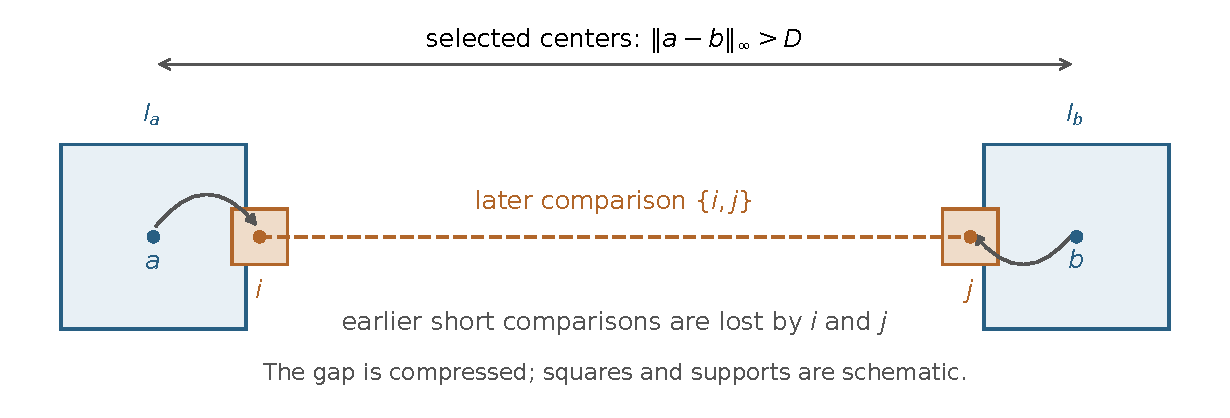
\includegraphics[width=\linewidth]{figures/separated-integrations.pdf}
 \caption{The geometry in Lemma~\ref{map:separated-integrations}, in
 parent units.  The orange supports meet the two selected squares.
 When $i\ne a$ and $j\ne b$, both endpoints have already lost a shorter
 comparison before the long comparison $\{i,j\}$.  If an endpoint
 equals its selected center, the proof uses the loss at the other
 endpoint.  Distances and support sizes are schematic; the separating
 gap is compressed.}
 \label{map:separation-figure}
\end{figure}

Given the new coins, collect all terms in
\eqref{map:coin-identity} meeting a selected $I_j$ into $H_j$.
Replace $H_j$ by
\begin{equation}\label{map:conditional-addition}
 \log\E_0[e^{H_j}\mid\text{field variables outside }I_j].
\end{equation}
All other terms remain.  The pure conditional laws in the selected
squares are independent given their exterior.  Lemma
\ref{map:separated-integrations} therefore shows, pointwise in the new
coins and exterior variables, that these replacements preserve the
integrated weight.  The output still contains every spin and old
auxiliary variable, together with the new coins; replacing the
logarithmic weight makes the updated old variables conditionally pure.
Their old law is recovered by the conditional tilt $e^{H_j}$.

Allocate a term in \eqref{map:conditional-addition} to its integration
parent.  Allocate untreated terms to their original parents, splitting
a pair term equally between its endpoints.  Fix these rules
symmetrically once and for all.  The allocated terms are functions of
the new coins as well as the remaining old field.  Center each by its
full-plane pure/reference mean.  The resulting potentials are denoted
$f'_j$.  Centering changes only a scalar partition factor, which can
depend on the environment but not on any field variable.

\begin{lemma}[Regular linearization]\label{map:linearization}
The regular map is analytic on a fixed supremum-norm neighborhood of
zero after $L$ is fixed.  Its derivatives of every prescribed finite
order are bounded uniformly in $s$ and depend on a bounded local
stencil of children.  Its first derivative is
\begin{equation}\label{map:linear-formula}
 f'_{j,\mathrm{lin}}
 =p^{-1}A_j\sum_{i\in\mathcal C_j}P^0_{I_j}f_i,
\end{equation}
where $P^0_{I_j}$ integrates the old reference field inside $I_j$.
The transferred sum is already centered.  In particular the linear
formula is independent of the reveal priorities.
\end{lemma}

\begin{proof}
Since $\E_eU_e=0$, every coin normalizer starts at degree two in the
child potentials.  The derivative of \eqref{map:conditional-addition}
at zero is conditional expectation.  These facts give
\eqref{map:linear-formula}.  Averaging the transfer in the full-plane
reference law gives zero by the centering of each child; averaging $A_j$
also preserves this centering.  On a small ball, real conditional
exponentials are uniformly bounded above and below.  The ordinary
power series for the exponential and logarithm consequently give the
asserted bounds in the supremum norm.  There are only finitely many
terms in each stencil, independently of $s$.
\end{proof}

\subsection{Large terms and isolated concentrations}

A moment estimate cannot assume that every realized potential is small.
We now modify the map where large child terms occur.  Fix $b>0$ and
independently attach to each child an environmental threshold uniform
on $[b,2b]$.  A child is a \emph{flag} if its norm exceeds its threshold.
The continuous thresholds will also make finite-step moment data
continuous in the initial coupling.

Declare a parent inactive when its center is within $10D$ parent units
of a flag.  In \eqref{map:coin-likelihood}, set its $F_j$ to zero and
retain its child terms separately.  Its coins remain as dummy
comparisons in the full local stars.  Active selected parents are
integrated as before.  Every retained term that involves an updated
interior variable is included in that integration; retained terms
supported entirely outside may simply be left in place.  Such a child
term has support much smaller than parent spacing and cannot meet two
selected squares.  Thus the same exact identity applies at the
boundary between active and inactive parents.

A further operation controls one isolated concentration of large terms.
Put $d_0=4C+10$.  An isolated group is a nonempty set $A$ of flags with
child-grid diameter at most $6d_0$ and with no flag outside $A$ within
$100D$ parent units of $A$.  Distinct such groups are separated.  Choose
one flag in $A$ using independent environmental priorities, and let
$j(A)$ be its parent.  Let
\[
 G_A=\sum_{i:\,\dist(i,A)\le3d_0}f_i,
 \qquad I_A=I_{j(A)}.
\]
Taking $L$ sufficiently large puts the support of $G_A$ deep inside
$I_A$.  All these children are in the inactive region.  No active
integration, or coin normalizer involving active old-field terms,
reaches $I_A$.

We remove $G_A$ while retaining all other interactions.  Let $B_A$ be
the sum of the remaining logarithmic terms that touch $I_A$.  With the
exterior fixed, replace $G_A$ by
\begin{equation}\label{map:isolated-ratio}
 R_A=\log\E_0[e^{B_A+G_A}\mid I_A^c]
       -\log\E_0[e^{B_A}\mid I_A^c].
\end{equation}
Here $I_A^c$ denotes all field variables not updated in $I_A$; new coins
are held fixed.  The identity
\begin{equation}\label{map:isolated-exactness}
 \E_0[e^{B_A+R_A}\mid I_A^c]
 =\E_0[e^{B_A+G_A}\mid I_A^c]
\end{equation}
proves that the exterior weight is unchanged.  The new conditional law
inside $I_A$ is tilted by $e^{B_A}$, and the old one by $e^{B_A+G_A}$.
In particular, retaining $B_A$ is part of the exact replacement.
Allocate $R_A$ to $j(A)$, and group all remaining terms at their parents.
These special integrations take priority over the preceding rule of
carrying inactive terms.  Their separation makes their order immaterial.

\begin{proposition}[The local scale map]\label{map:step}
There is a fixed support constant $C$ such that, for all sufficiently
large odd $L$ and every $b>0$, the preceding construction maps a field
with spacing $s$ and support/dependence radius $Cs$ to a field with
spacing $s'=Ls$ and support/dependence radius $Cs'$.  Its outputs are
centered, spin-flip even, stationary on the parent grid, and square
symmetric in distribution.  For a fixed numerical $K$ and a constant
$C_L$,
\begin{equation}\label{map:raw-bound}
 \|f'_j\|\le C_L\sum_{i:\,\|si-s'j\|_\infty\le Ks'}\|f_i\|.
\end{equation}
All replacements preserve exterior-integrated weights exactly, up to
the scalar constants removed by centering, and admit the reversals
described above.  The same formulas and centering constants apply in
embedded plane and torus charts.
\end{proposition}

\begin{proof}
Choose $C$ large enough to contain the comparison, inactivity, and
isolation ranges in parent units.  Then choose $L$ so large that old
supports overhang a parent by less than $1/10$ parent unit and
$100d_0/L<1/10$.  Every selection or status check, local allocation, and
conditional partition function then uses a fixed parent stencil.
Old environment dependence adds only an overhang $C/L$ in these units.
The new priorities and thresholds are independent and located in the
same stencil.  Increasing $C$ once, before fixing $L$, covers all these
supports.  No integration requires environment variables beyond the
terms that touch its finite square.

For any probability kernel $P$ and real bounded $H$,
$|\log Pe^H|\le\|H\|$.  The same inequality and its Lipschitz version
bound \eqref{map:conditional-addition} and
\eqref{map:isolated-ratio} by sums of the input norms.  The factors
$p^{-1}$ and the finite numbers of terms depend only on the fixed step.
Centering at most doubles this bound, proving \eqref{map:raw-bound}.
Spin flip commutes with every operation.  The symmetric choices and
allocation rules give the stated invariance in distribution.
Exactness follows from the normalized decoration,
\eqref{map:conditional-addition}, and
\eqref{map:isolated-exactness}.  Pure conditional kernels in an embedded
square depend only on its boundary assignment, so the same identities
hold on a torus.  We always subtract the same full-plane centering
constants, rather than torus means.
\end{proof}

\begin{corollary}[Local implementation]\label{map:locality}
In a finite free chart $W$ with arbitrary exterior field data, the map
can be performed away from its boundary so that the resulting
specification agrees with the full scale-$s'$ specification in
$W$ eroded by $K_1s'$, for a fixed numerical $K_1$.
\end{corollary}

\begin{proof}
Use the full local comparison stars.  If a parent's complete decoration
and allocation stencil leaves $W$, set its $F_j$ to zero in every $U_e$
and retain its original child logs separately.  Thus every fresh coin
with a nontrivial likelihood is inside $W$ and is sampled.  Skip integrations
whose stencils leave $W$.  Include retained terms in any
interior integration they meet.  Skip special integrations near the
boundary and keep active ones separated from them as above.  Every
operation affecting the eroded chart then uses precisely its full
stencil.  All remaining discrepancies are supported in the removed
boundary layer.  The argument applies also to annular charts.
\end{proof}

\subsection{Reversing the map and measuring finite insertions}

\begin{proposition}[A coupling of consecutive fields]\label{map:reversal}
For each fixed environment, the input and output spin fields of the
torus construction, or of the local construction with prescribed old
exterior field variables, can be
coupled so that they agree outside squares of radius $5s'$ about marked
parent centers.  The marks are mutually independent conditional on the
environment, independent of the output Gibbs sample, and have local
environmental parameters $p_j$ satisfying
\begin{equation}\label{map:mark-parameter}
 p_j\le\min\left\{1,C_L
       \sum_{i:\,\|si-s'j\|_\infty\le Ks'}\|f_i\|\right\}.
\end{equation}
For any $P\ge1$ and a stationary field with a finite $P$th environmental moment,
$\E p_j\le C_L(\E\|f_0\|^P)^{1/P}$.  These conclusions hold uniformly
over the old exterior assignments in the local implementation of
Corollary~\ref{map:locality}.
\end{proposition}

\begin{proof}
First sample the entire output Gibbs field, including the new coins.
Independently sample a uniform variable at every candidate parent
center, and mark $j$ when it is at most
$p_j=1-e^{-C_LS_j}$, with $S_j$ the environmental norm sum in
\eqref{map:mark-parameter}.  These parameters depend only on the
environment, so the marks have exactly the independence stated in the
proposition, before any further conditioning.

Condition now on the new coins and the common exterior of the updated
squares.  The ratio of the old conditional density to the new one is
bounded below by $e^{-C_LS_j}$, where $S_j$ is the local norm sum in
\eqref{map:mark-parameter}.  This follows from the real log bounds used
in Proposition~\ref{map:step}; for a special square it applies to the
tilt from $B_A$ to $B_A+G_A$.  If two laws satisfy
$\mu\ge(1-p)\nu$ and $p>0$, sample from $\nu$, retain that sample with probability
$1-p$, and otherwise sample from
$[\mu-(1-p)\nu]/p$.  The Bernoulli decision can be independent of the
$\nu$ sample; when $p=0$ the laws agree and the sample is retained.
Use this residual resampling in each marked updated square.  Conditional
factorization over the separated squares proves that the resampled
field has the old conditional law.  Unused centers keep their dummy
marks and cause no change.  Each update lies inside its radius-$5s'$ square.
Finally discard the conditionally decorated coins.  Their decoration
was normalized at each old field, so this recovers the input marginal.
Taking environmental expectation in \eqref{map:mark-parameter} gives
the last bound.
\end{proof}

One further consequence of exactness is needed for the variance
calculation.  For a finite family of labeled potentials at scale $s$,
define its normalized insertion density and charge by
\[
 D_f=\frac{\exp(\sum_i f_i)}{\E_0\exp(\sum_i f_i)},
 \qquad T_s(f)=q_s(D_f).
\]
The following statement concerns the regular map, before flags are
introduced, and therefore also its Taylor coefficients at zero.

\begin{corollary}[Charge of a finite insertion]\label{map:insertion-charge}
For every finite family of input labels, each fixed environment, and
each realization of the reveal priorities, the regular map satisfies
\[
 T_{Ls}(f')=L^{-1}T_s(f).
\]
The identity holds coefficientwise when separate indeterminates are
attached to the input labels.
\end{corollary}

\begin{proof}
Only a finite neighborhood of the insertion has nonzero decorations or
replacement terms.  Every observable outside a larger buffered region
has the same expectation against the normalized input and output
densities, because the decorations and replacements preserve its
unnormalized pairing and the partition function.  Apply this to a pure
bond tending to infinity.  Theorem~\ref{pure:charge} identifies the
limiting pairing with $Q$, so the total lattice charge is unchanged.
Dividing by the output scale $Ls$ instead of $s$ gives the factor
$L^{-1}$.  Scalar centering constants cancel in $D_f$.  Analyticity near
zero gives the coefficientwise assertion.
\end{proof}
